\subsubsection{05.01.2016}
\textit{\textbf{Time frame:}} 17:00-21:30 \newline
The mechanism for shifting the bucket was finished.

The assembling of the new version of the mechanism for scoring autonomous alpinists was started (figure \ref{Alpinists2.1}, \ref{Alpinists2.2}, \ref{Alpinists2.3}).

\begin{figure}[H]
	\begin{minipage}[h]{0.31\linewidth}
		\center{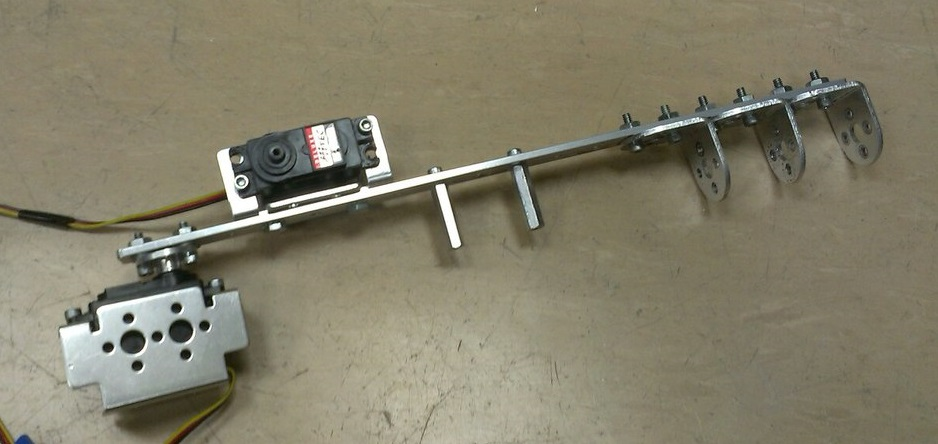
\includegraphics[scale=0.17]{3Engineering/5Team_meetings/days_of_meetings/2016.01.05/images/01}}
		\caption{New mechanism for scoring alpinists}
		\label{Alpinists2.1}
	\end{minipage}
	\hfill
	\begin{minipage}[h]{0.31\linewidth}
		\center{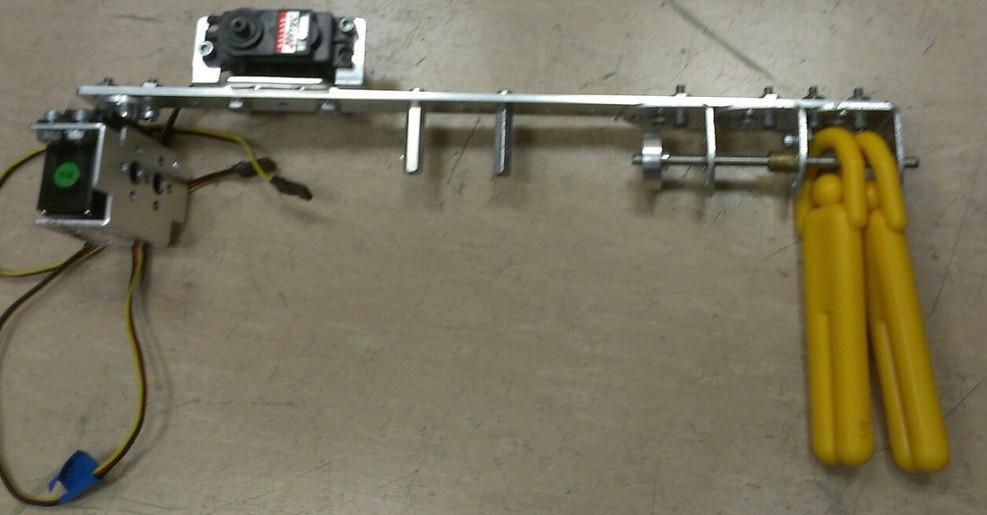
\includegraphics[scale=0.15]{3Engineering/5Team_meetings/days_of_meetings/2016.01.05/images/02}}
		\caption{How does it work 1}
		\label{Alpinists2.2}
	\end{minipage}
	\hfill
	\begin{minipage}[h]{0.31\linewidth}
		\center{
\includegraphics[scale=0.15]{3Engineering/5Team_meetings/days_of_meetings/2016.01.05/images/03}}
		\caption{How does it work 2}
		\label{Alpinists2.3}
	\end{minipage}
\end{figure}

2 standard TETRIX motors at the winch were replaced with 3 NeveRest AndyMark motors (figure \ref{Winch2.8}). Firstly, it 2 times increased torque at the coil (3 AndyMarks give torque of $3 \cdot 25 = 75 kg \cdot cm$, while 2 standard - only $2 \cdot 20 = 40 kg \cdot cm$). Secondly, it raised the reliability of the construction, as the AndyMark motors can cope with stalling for a long time (about 2 minutes), so they will not break down if the movement of the elevator is blocked.

\begin{figure}[H]
	\begin{minipage}[h]{1\linewidth}
		\center{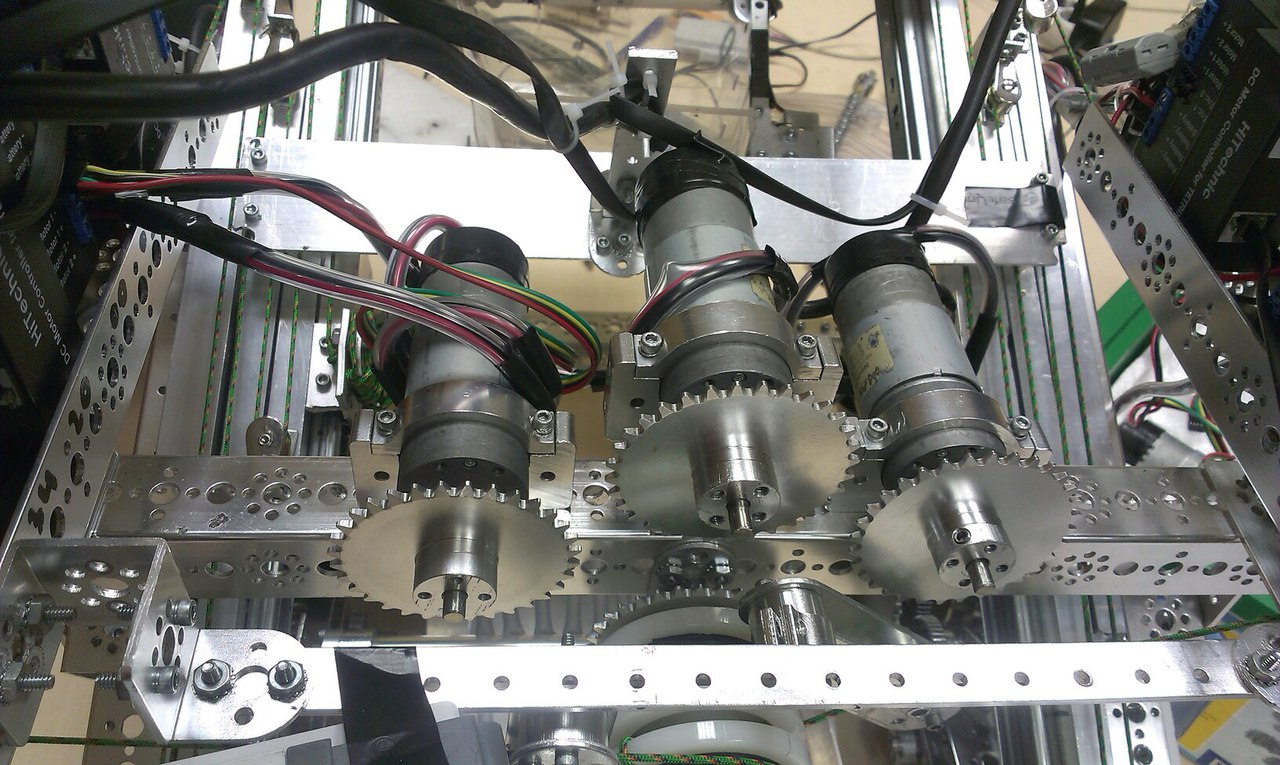
\includegraphics[scale=0.2]{3Engineering/5Team_meetings/days_of_meetings/2016.01.05/images/04}}
		\caption{Three motors for powering the winch are installed}
		\label{Winch2.9}
	\end{minipage}
\end{figure}

